%package list
\documentclass{article}
\usepackage[top=3cm, bottom=3cm, outer=3cm, inner=3cm]{geometry}
\usepackage{multicol}
\usepackage{graphicx}
\usepackage{url}
%\usepackage{cite}
\usepackage{hyperref}
\usepackage{array}
%\usepackage{multicol}
\newcolumntype{x}[1]{>{\centering\arraybackslash\hspace{0pt}}p{#1}}
\usepackage{natbib}
\usepackage{pdfpages}
\usepackage{multirow}
\usepackage[normalem]{ulem}
\useunder{\uline}{\ul}{}
\usepackage{svg}
\usepackage{xcolor}
\usepackage{listings}
\lstdefinestyle{ascii-tree}{
    literate={├}{|}1 {─}{--}1 {└}{+}1 
  }
\lstset{basicstyle=\ttfamily,
  showstringspaces=false,
  commentstyle=\color{red},
  keywordstyle=\color{blue}
}
%\usepackage{booktabs}
\usepackage{caption}
\usepackage{subcaption}
\usepackage{float}
\usepackage{array}

\newcolumntype{M}[1]{>{\centering\arraybackslash}m{#1}}
\newcolumntype{N}{@{}m{0pt}@{}}


%%%%%%%%%%%%%%%%%%%%%%%%%%%%%%%%%%%%%%%%%%%%%%%%%%%%%%%%%%%%%%%%%%%%%%%%%%%%
%%%%%%%%%%%%%%%%%%%%%%%%%%%%%%%%%%%%%%%%%%%%%%%%%%%%%%%%%%%%%%%%%%%%%%%%%%%%
\newcommand{\itemEmail}{fayamamani@unsa.edu.pe}
\newcommand{\itemStudent}{Francis Willian Ayamamani Añasco}
\newcommand{\itemCourse}{Programación Web 2}
\newcommand{\itemCourseCode}{GUIA-PRLD-001}
\newcommand{\itemSemester}{I}
\newcommand{\itemUniversity}{Universidad Nacional de San Agustín de Arequipa}
\newcommand{\itemFaculty}{Facultad de Ingeniería de Producción y Servicios}
\newcommand{\itemDepartment}{Departamento Académico de Ingeniería de Sistemas e Informática}
\newcommand{\itemSchool}{Escuela Profesional de Ingeniería de Sistemas}
\newcommand{\itemAcademic}{2023 - A}
\newcommand{\itemInput}{Del 30 Junio 2023}
\newcommand{\itemOutput}{Al 30 Junio 2023}
\newcommand{\itemPracticeNumber}{05}
\newcommand{\itemTheme}{Django-PARTE I}
%%%%%%%%%%%%%%%%%%%%%%%%%%%%%%%%%%%%%%%%%%%%%%%%%%%%%%%%%%%%%%%%%%%%%%%%%%%%
%%%%%%%%%%%%%%%%%%%%%%%%%%%%%%%%%%%%%%%%%%%%%%%%%%%%%%%%%%%%%%%%%%%%%%%%%%%%

\usepackage[english,spanish]{babel}
\usepackage[utf8]{inputenc}
\AtBeginDocument{\selectlanguage{spanish}}
\renewcommand{\figurename}{Figura}
\renewcommand{\refname}{Referencias}
\renewcommand{\tablename}{Tabla} %esto no funciona cuando se usa babel
\AtBeginDocument{%
	\renewcommand\tablename{Tabla}
}

\usepackage{fancyhdr}
\pagestyle{fancy}
\fancyhf{}
\setlength{\headheight}{30pt}
\renewcommand{\headrulewidth}{1pt}
\renewcommand{\footrulewidth}{1pt}
\fancyhead[L]{\raisebox{-0.2\height}{
\includegraphics[width=3cm]{img/logo_episunsa.png}}}
\fancyhead[C]{\fontsize{7}{7}\selectfont	\itemUniversity \\ \itemFaculty \\ \itemDepartment \\ \itemSchool \\ \textbf{\itemCourse}}
\fancyhead[R]{\raisebox{-0.2\height}{
\includegraphics[width=1.2cm]{img/logo_abet}}}
\fancyfoot[L]{Estudiante Francis Ayamamani Añasco}
\fancyfoot[C]{\itemCourse}
\fancyfoot[R]{Página \thepage}

% para el codigo fuente
\usepackage{listings}
\usepackage{color, colortbl}
\definecolor{dkgreen}{rgb}{0,0.6,0}
\definecolor{gray}{rgb}{0.5,0.5,0.5}
\definecolor{mauve}{rgb}{0.58,0,0.82}
\definecolor{codebackground}{rgb}{0.95, 0.95, 0.92}
\definecolor{tablebackground}{rgb}{0.8, 0, 0}

\lstset{frame=tb,
	language=bash,
	aboveskip=3mm,
	belowskip=3mm,
	showstringspaces=false,
	columns=flexible,
	basicstyle={\small\ttfamily},
	numbers=none,
	numberstyle=\tiny\color{gray},
	keywordstyle=\color{blue},
	commentstyle=\color{dkgreen},
	stringstyle=\color{mauve},
	breaklines=true,
	breakatwhitespace=true,
	tabsize=3,
	backgroundcolor= \color{codebackground},
}

\begin{document}
	
	\vspace*{10px}
	
	\begin{center}	
		\fontsize{17}{17} \textbf{ Informe de Laboratorio \itemPracticeNumber}
	\end{center}
	\centerline{\textbf{\Large Tema: \itemTheme}}
	%\vspace*{0.5cm}	

	\begin{flushright}
		\begin{tabular}{|M{2.5cm}|N|}
			\hline 
			\rowcolor{tablebackground}
			\color{white} \textbf{Nota}  \\
			\hline 
			     \\[30pt]
			\hline 			
		\end{tabular}
	\end{flushright}	

	\begin{table}[H]
		\begin{tabular}{|x{4.7cm}|x{4.8cm}|x{4.8cm}|}
			\hline 
			\rowcolor{tablebackground}
			\color{white} \textbf{Estudiante} & \color{white}\textbf{Escuela}  & \color{white}\textbf{Asignatura}   \\
			\hline 
			{\itemStudent \par \itemEmail} & \itemSchool & {\itemCourse \par Semestre: \itemSemester \par Código: \itemCourseCode}     \\
			\hline 			
		\end{tabular}
	\end{table}		
	
	\begin{table}[H]
		\begin{tabular}{|x{4.7cm}|x{4.8cm}|x{4.8cm}|}
			\hline 
			\rowcolor{tablebackground}
			\color{white}\textbf{Laboratorio} & \color{white}\textbf{Tema}  & \color{white}\textbf{Duración}   \\
			\hline 
			\itemPracticeNumber & \itemTheme & 04 horas   \\
			\hline 
		\end{tabular}
	\end{table}
	
	\begin{table}[H]
		\begin{tabular}{|x{4.7cm}|x{4.8cm}|x{4.8cm}|}
			\hline 
			\rowcolor{tablebackground}
			\color{white}\textbf{Semestre académico} & \color{white}\textbf{Fecha de inicio}  & \color{white}\textbf{Fecha de entrega}   \\
			\hline 
			\itemAcademic & \itemInput &  \itemOutput  \\
			\hline 
		\end{tabular}
	\end{table}
	
	\section{Tarea}
	\begin{itemize}
		\item Creacion del sitio respecto al administrador:
        \begin{enumerate}
            \item Creacion del models.py
            \item Creacion de las funciones de views.py
            \item Creacion de Templates
            \item Vincular las rutas en urls.py
        \end{enumerate}
        \end{itemize}
	\section{MARCO CONCEPTUAL}
	\begin{itemize}
		\item Editor Vim
        \begin{itemize}
            \item Vim es un editor de texto muy eficiente para programar en consola que no tiene nada que envidiar a los editores gráficos.
        \end{itemize}
        \item Instalar Vim en
        \begin{itemize}
            \item GNU/Linux
                \begin{lstlisting}
                    apt-get install vim
                \end{lstlisting}
            \item MS Windows
            \begin{itemize}
                \item Para descarga en sistemas MS Windows \url{https://www.vim.org/download.php}
            \end{itemize}
            \item MacOS
                \begin{lstlisting}
                    brew install macvim
                \end{lstlisting}
        \item Git
        \begin{itemize}
            \item Git es un sistema de control de versiones creado por Linus Torvalds. Es eficiente, confiable.
        \end{itemize}
        \item Instalar Git
        \begin{itemize}
            \item GNU/Linux
                \begin{lstlisting}
                apt-get install git    
                \end{lstlisting}
            \item MS Windows
            \begin{itemize}
                \item Para descarga en sistemas MS Windows \url{https://git-scm.com/download/win}
            \end{itemize}
            \item MacOS
            \begin{itemize}
                \item Para descarga en sistemas MacOS \url{https://git-scm.com/download/mac}
                \begin{lstlisting}
                    brew install git
                \end{lstlisting}
            \end{itemize}
        \end{itemize}
        \item python
        \begin{itemize}
            \item Para un instalación local en sistemas operativos MS Windows utilice: https://www.python.org/downloads/windows/
            \item Tambien ud puede probar código en herramientas online: \url{https://www.programiz.com/python-programming/online-compiler/}
            \item Python en Debian GNU/Linux:
            \begin{itemize}
            \begin{lstlisting}[language=bash,caption={Debian Linux viene con Python 3 y Python 2 preinstalados.}][H]
		          python3 --version
                    Python 3.9.2
	        \end{lstlisting}
            \begin{lstlisting}[language=bash,caption={Instalemos pip, una herramienta que instalará y administrará los paquetes de programación que queramos usar en nuestros proyectos de desarrollo.}][H]
		          sudo apt-get install -y python3-pip
	        \end{lstlisting}
            \begin{lstlisting}[language=bash,caption={Paquetes y herramientas de desarrollo más para instalar para garantizar que tengamos una configuración sólida para nuestro entorno de programación:}][H]
		          sudo apt-get install build-essential libssl-dev libffi-dev python3-dev
	        \end{lstlisting}
            \item Configurar un entorno virtual:
                \item Los entornos virtuales permiten tener un espacio aislado en los proyectos Python
                \item Garantizando que cada proyecto pueda tener su propio conjunto de dependencias que no interrumpirán a otros proyectos.
                \item Manejando diferentes versiones de los paquetes. Esto es especialmente importante cuando se trabaja con paquetes de terceros.
                \item Puede varios entornos de programación.
                \item Cada entorno es un directorio en la que se ubicaran sus scripts.
                \item Usaremos el módulo venv , que es parte de la biblioteca estándar de Python.
                \begin{lstlisting}[language=bash,caption={Entorno de Linux-Instalemos venv escribiendo:}][H]
    		          sudo apt install -y python3-venv
    	        \end{lstlisting}
                \begin{lstlisting}[language=bash,caption={Entorno de Linux-Para crear un ambiente elija en qué directorio.}][H]
    		          mkdir -p ~/unsa/pw2/labs/lab04/entorno
                        cd ~/unsa/pw2/labs/lab04/entorno
    	        \end{lstlisting}
                \begin{lstlisting}[language=bash,caption={Entorno de Linux-En el directorio crea un entorno virtual ejecutando el siguiente comando:}][H]
    		          virtualenv -p python3 .
    	        \end{lstlisting}
                \begin{lstlisting}[language=bash,caption={Entorno de Linux-Ejecute el script de activación para activar el entorno virtual:}][H]
    		          source ../bin/activate
    	        \end{lstlisting}
            \end{itemize}
        \end{itemize}
	\end{itemize}
	
	\section{URL de Repositorio Github}
	\begin{itemize}
		\item URL del Repositorio GitHub para clonar o recuperar.
		\item \url{https://github.com/rescobedoq/pw2/tree/main/labs/lab05}
		\item URL para el laboratorio 05 en el Repositorio GitHub.
		\item \url{https://github.com/rescobedoq/pw2/tree/main/labs/lab05}
	\end{itemize}
	
	\section{Resolucion de la tarea}
    \subsection{Inicio}
    \begin{itemize}
        \item Creacion de la carpeta de Trabajo
        \begin{lstlisting}[language=bash,caption={Entorno de Linux-Ejecute el script de activación para activar el entorno virtual:}][H]
    		          mkdir PWB
    	\end{lstlisting}
        \item Activar el entorno virtual
        \begin{lstlisting}[language=bash,caption={Entorno de Linux-Ejecute el script de activación para activar el entorno virtual:}][H]
    		          source {{Direccion de tu entorno Virtual}}
    	\end{lstlisting}
         \item Gestionar las versiones instaladas
        \begin{lstlisting}[language=bash,caption={Entorno de Linux-Ejecute el script de activación para activar el entorno virtual:}][H]
    		          pip list
    	\end{lstlisting}
        \item Instalar django
        \begin{lstlisting}[language=bash,caption={Entorno de Linux-Ejecute el script de activación para activar el entorno virtual:}][H]
    		          pip install Django
    	\end{lstlisting}
        \item Verificas
        \begin{lstlisting}[language=bash,caption={Entorno de Linux-Ejecute el script de activación para activar el entorno virtual:}][H]
    		          pip list
                    //resultado:
                        Package    Version
                        ---------- -------
                        asgiref    3.5.2
                        Django     4.0.5 //Variable
                        pip        22.0.4
                        setuptools 62.1.0
                        sqlparse   0.4.2
                        wheel      0.37.1
    	\end{lstlisting}
        \item Crear el projecto
        \begin{lstlisting}[language=bash,caption={Entorno de Linux-Ejecute el script de activación para activar el entorno virtual:}][H]
    		          django-admin startproject {{nombre_del_proyecto}}
    	\end{lstlisting}
        \item RESULTADO
        \begin{lstlisting}[style=ascii-tree]
        PWB/
        |--- manage.py
        |--- PWB/
            |   |--- __init__.py
            |   |--- asgi.py
            |   |--- settings.py
            |   |--- urls.py
        \end{lstlisting}
        \item Crear el APP para el funcionamiento de una parte del projecto
        \begin{lstlisting}[language=bash,caption={Entorno de Linux-Ejecute el script de activación para activar el entorno virtual:}][H]
    		          python manage.py startapp {{nombre_app}}
    	\end{lstlisting}
        \item RESULTADO
        \begin{lstlisting}[style=ascii-tree]
        PWB/
        |--- manage.py
        #nombre de mi APP
        |--- Decoraciones/
            |   |--- migration
            |   |--- __init__.py
            |   |--- admin.py
            |   |--- apps.py
            |   |--- models.py
            |   |--- tests.py
            |   |--- views.py
            |   |--- urls.py
        |--- PWB/
            |   |--- __init__.py
            |   |--- asgi.py
            |   |--- settings.py
            |   |--- urls.py
        \end{lstlisting}
    \end{itemize}
	\subsection{Explicacion del Codigo}
    \begin{lstlisting}[language=python,caption={Decoraciones/models.py}][H]
from django.db import models

class Tipo(models.Model):
    Tip = models.CharField(max_length=50, default=None, null=True)

    def __str__(self):
        return self.Tip
    
class Producto(models.Model):
    nombre = models.CharField(max_length=25)
    descripcion = models.TextField()
    precio = models.CharField(max_length=25)

    class Meta:
        abstract = True

class catalogo(Producto):
    imagen = models.ImageField(null=True, blank=True, upload_to="img/")
    tipo = models.ForeignKey(Tipo, on_delete=models.CASCADE, null=True)

    def __str__(self):
        return self.nombre

class Carrito(Producto):
    adquirido = models.BooleanField()
    rutaI = models.CharField(null=True, max_length=50000)
    
class Pedido(models.Model):
    NombreC = models.CharField(null=True, max_length=50)
    ApellidosC = models.CharField(null=True, max_length=50)
    telefono = models.IntegerField(null=True)
    Correo = models.EmailField(max_length=254, default='')
    direccion = models.CharField(max_length=50)
    fecha = models.DateField()
    Carrito = models.ForeignKey(Carrito, on_delete=models.CASCADE, null=True)

    \end{lstlisting}
	\begin{itemize}
	    \item \textbf{Tipo}: Es un modelo que representa el tipo de producto. Tiene un campo Tip que es un CharField de máximo 50 caracteres de la cadena de texto. La función\textbf{str} devuelve la vista del admin, este caso sería el valor del campo Tip.
        \item \textbf{Producto}: Es una clase abstracta que representa un producto genérico. Tiene tres campos: nombre, descripcion y precio. Estos campos son un CharField, un TextField y otro CharField respectivamente. Al declarar \textbf{abstract = True} en la clase Meta, se indica que este modelo es abstracto.
        \item \textbf{catalogo}: Este hereda de Producto y representa un producto en particular.Integra un campo imagen que es un ImageField para almacenar la imagen del producto, y un campo tipo que es una clave externa (\textbf{ForeignKey}) que se relaciona con el modelo Tipo.
        \item \textbf{Carrito}: Es un modelo que también hereda de Producto y representa un producto agregado al carrito de compras. Además de los campos heredados de Producto, tiene un campo adquirido que es un BooleanField para indicar si el producto ha sido adquirido, y un campo rutaI que es un CharField para almacenar la ruta de la imagen del producto.
        \item \textbf{Pedido}: Es un modelo que representa un pedido realizado por un cliente. Tiene varios campos como NombreC, ApellidosC, telefono, Correo, direccion, fecha y Carrito. Estos campos representan información relacionada con el pedido, como el nombre del cliente, apellidos, teléfono, correo, dirección, fecha del pedido, y un campo Carrito que es una clave externa (ForeignKey) que se relaciona con el modelo Carrito.
	\end{itemize}
     \begin{lstlisting}[language=python,caption={Decoraciones/models.py}][H]
from django.contrib import admin
from Decoraciones.models import Pedido,catalogo,Carrito,Tipo
# Register your models here.
admin.site.register(Tipo)
admin.site.register(Pedido)
admin.site.register(catalogo)
admin.site.register(Carrito)
    \end{lstlisting}
	\begin{itemize}
	    \item\textbf{La línea from django.contrib import admin} importa el módulo admin de Django, que proporciona las funcionalidades relacionadas con el panel de administración.
        \item Luego se importan los modelos Pedido, catalogo, Carrito y Tipo desde el módulo models de la aplicación Decoraciones.
        \item La función \textbf{admin.site.register(Modelo)} se utiliza para registrar cada modelo en el panel de administración. Aquí, se registran los modelos Tipo, Pedido, catalogo y Carrito.
	\end{itemize}
    \begin{lstlisting}[language=python,caption={Decoraciones/views.py}][H]
from django.shortcuts import render
from Decoraciones.models import catalogo
# Lista de elementos
list_producto=catalogo.objects.all()
#Pagina de Inicio
def Home(request):
    return render(request,"home.html",{"producs":list_producto})
def Bebidas(request):
    return render(request,"Bbs.html",{"producs":list_producto})
def Bocaditos(request):
    return render(request,"Bts.html",{"producs":list_producto})
def Equipos(request):
    return render(request,"Eps.html",{"producs":list_producto})
def Decoraciones(request):
    return render(request,"Dec.html",{"producs":list_producto})
    \end{lstlisting}
	\begin{itemize}
	    \item \textbf{from Decoraciones.models import catalogo}.Importa el modelo catalogo desde el archivo models.py del directorio Decoraciones. Esto permite acceder a los objetos de la clase catalogo definida en ese modelo.
        \item \textbf{$list_producto$=catalogo.objects.all()}, obtiene todos los objetos de la clase catalogo almacenados y los asigna a la variable \textbf{$list_producto$}. Esto devuelve una lista de todos los productos.
        \item \textbf{def Home(request)}, es una función que recibe un objeto request como parámetro. Esta función se utiliza para manejar el template \textbf{home.html}.
        \item \textbf{return render(request,"home.html",{"producs":$list_producto$})}, renderiza la plantilla home.html y la devuelve como respuesta HTTP. Además, se pasa un diccionario como contexto a la plantilla, donde la clave "producs" es $list_producto$. Esto permite acceder a la lista de productos en la plantilla para mostrarlos.
        \item Las funciones Bebidas, Bocaditos, Equipos y Decoraciones siguen la misma estructura que la función Home. Cada una maneja una solicitud específica para mostrar una página correspondiente a cada una de ellas.
    \end{itemize}
	\begin{lstlisting}[language=python,caption={Decoraciones/urls.py}][H]
from django.urls import path
from Decoraciones import views
urlpatterns = [
    path('', views.Home, name="Inicio"),
    path('Bebidas/', views.Bebidas, name="Bebidas"),
    path('Bocaditos/', views.Bocaditos, name="Bocaditos"),
    path('Equipos/', views.Equipos, name="Equipos"),
    path('Decoraciones/', views.Decoraciones, name="Decoraciones"),
]
    \end{lstlisting}
	\begin{itemize}
	    \item \textbf{urlpatterns = [...]}, es una lista que contiene todas las rutas URL de la aplicación y las funciones de vista asociadas a cada una.
        \item \textbf{path('', views.Home, name="Inicio")}, define una ruta URL vacía ('') que corresponde a la página de inicio de la aplicación. Asocia esta ruta con la función de vista Home del módulo views. Además, le asigna el nombre "Inicio" a esta ruta, lo que permite referenciarla fácilmente en otros lugares del código.
        \item Y de igual manera path('Bebidas/','Bocaditos/','Equipos/','Decoraciones/').Definen una ruta URL que corresponde a una parte de la página de decoraciones de la aplicación. Asocia esta ruta con la funcion correspondiente y le asigna el nombre "Decoraciones"..
    \end{itemize}
    \subsection{Ejecucion}
        \begin{figure}[H]
		          \centering
		          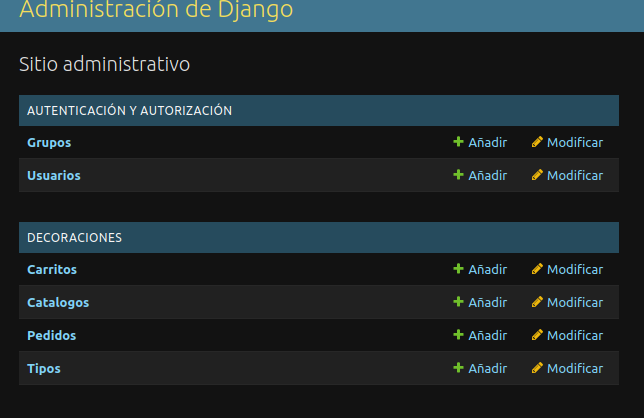
\includegraphics[scale=0.4,keepaspectratio]{img/Captura desde 2023-06-30 19-12-00.png}
		          %\includesvg{img/automata.svg}
		          %\label{img:mot2}
		          %\caption{Product backlog.}
	            \end{figure}
    \begin{itemize}
        \item En este caso se observa el administrador con todas las clases de models.py
    \end{itemize}
        \begin{figure}[H]
		          \centering
		          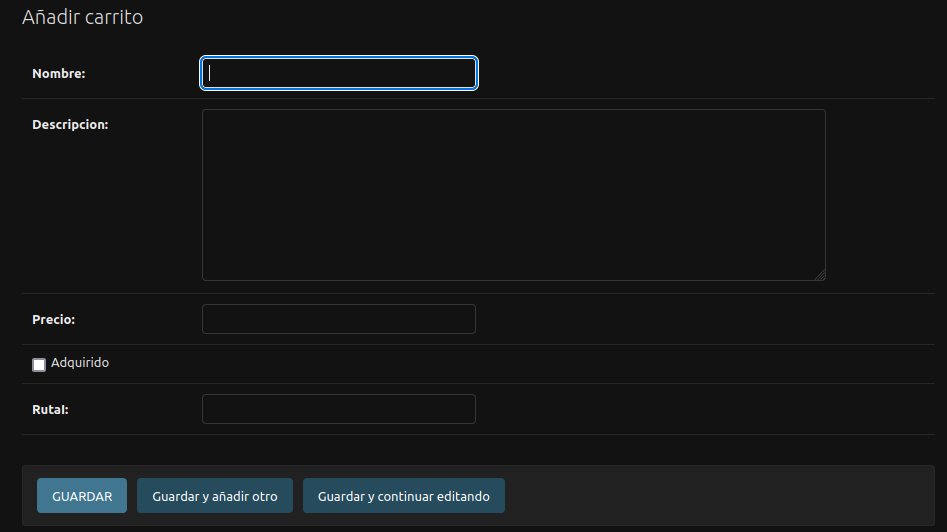
\includegraphics[scale=0.4,keepaspectratio]{img/Captura desde 2023-06-30 19-48-36.png}
		          %\includesvg{img/automata.svg}
		          %\label{img:mot2}
		          %\caption{Product backlog.}
	            \end{figure}
    \begin{itemize}
        \item En este caso se observa el administrador con la vista del formulacio de la clase Carritos de models.py
    \end{itemize}
            \begin{figure}[H]
		          \centering
		          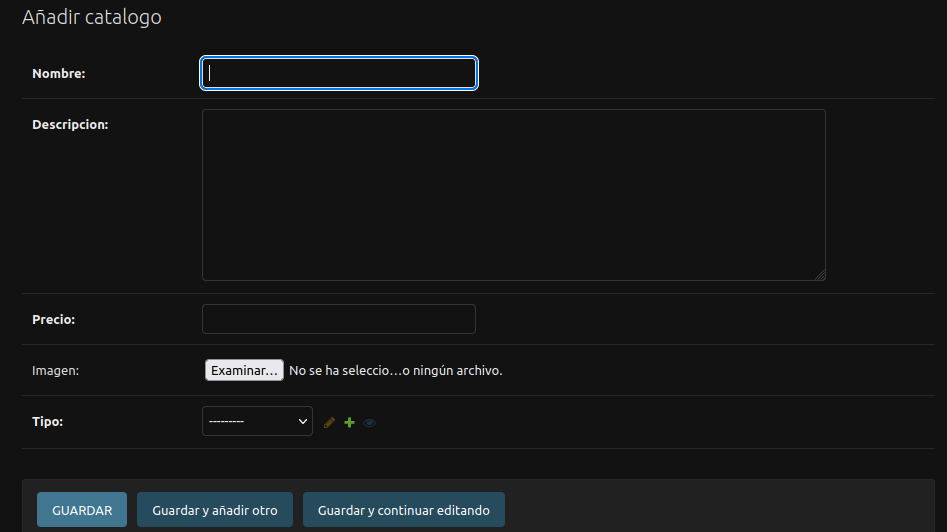
\includegraphics[scale=0.4,keepaspectratio]{img/Captura desde 2023-06-30 19-50-37.png}
		          %\includesvg{img/automata.svg}
		          %\label{img:mot2}
		          %\caption{Product backlog.}
	            \end{figure}
    \begin{itemize}
        \item En este caso se observa el administrador con la vista del formulacio de la clase Catalogos de models.py
    \end{itemize}
    \begin{figure}[H]
		          \centering
		          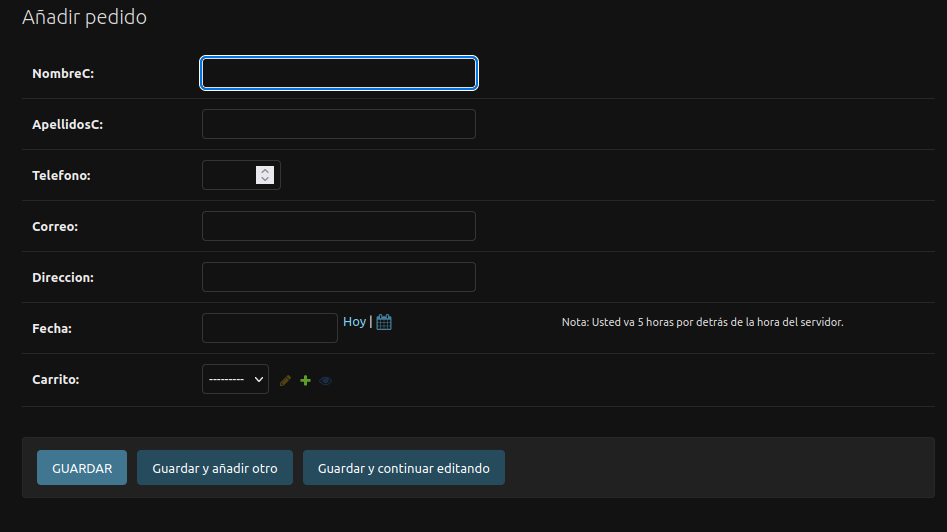
\includegraphics[scale=0.4,keepaspectratio]{img/Captura desde 2023-06-30 19-55-03.png}
		          %\includesvg{img/automata.svg}
		          %\label{img:mot2}
		          %\caption{Product backlog.}
	            \end{figure}
    \begin{itemize}
        \item En este caso se observa el administrador con la vista del formulacio de la clase Pedidos de models.py
    \end{itemize}
        \begin{figure}[H]
		          \centering
		          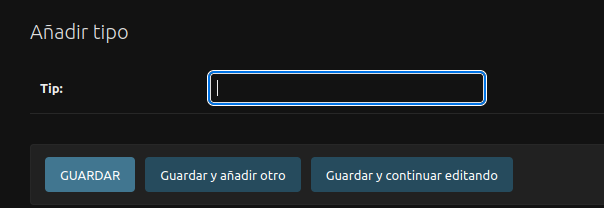
\includegraphics[scale=0.4,keepaspectratio]{img/Captura desde 2023-06-30 19-56-32.png}
		          %\includesvg{img/automata.svg}
		          %\label{img:mot2}
		          %\caption{Product backlog.}
	            \end{figure}
    \begin{itemize}
        \item En este caso se observa el administrador con la vista del formulacio de la clase Tipos de models.py
    \end{itemize}
    \section{Commit-Estructura}
    \subsection{Commit-Laboratorio 05}
    \begin{figure}[H]
		          \centering
		          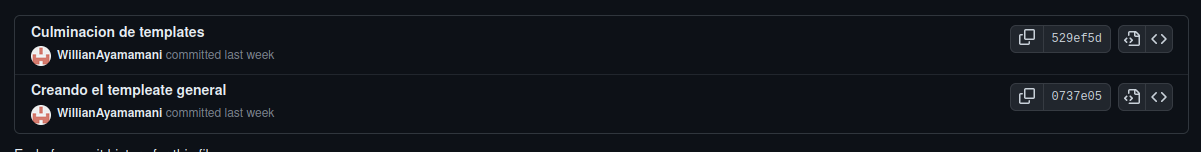
\includegraphics[scale=0.4,keepaspectratio]{img/Captura desde 2023-06-30 20-16-57.png}
		          %\includesvg{img/automata.svg}
		          %\label{img:mot2}
		          %\caption{Product backlog.}
	\end{figure}
    \begin{figure}[H]
		          \centering
		          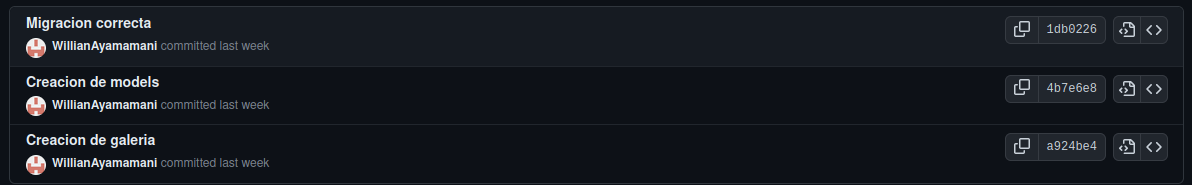
\includegraphics[scale=0.4,keepaspectratio]{img/Captura desde 2023-06-30 20-17-33.png}
		          %\includesvg{img/automata.svg}
		          %\label{img:mot2}
		          %\caption{Product backlog.}
	\end{figure}
	\subsection{Estructura de laboratorio 05}
	\begin{itemize}	
		\item El contenido que se entrega en este laboratorio es el siguiente:
	\end{itemize}
\begin{lstlisting}[style=ascii-tree]
lab5/
|--- LATEX/
    |   |--- main.tex
    |   |--- lab5.pdf
    |   |--- img
            |   |--- .gitignore
            |   |--- Captura desde 2023-06-30 18-12-00.png
            |   |--- Captura desde 2023-06-30 18-12-00.png
            |   |--- Captura desde 2023-06-30 18-12-00.png
            |   |--- Captura desde 2023-06-30 18-12-00.png
            |   |--- Captura desde 2023-06-30 18-12-00.png
            |   |--- Ejercicio2e.py
            |   |--- Ejercicio2f.py
            |   |--- Ejercicio2g.py
            |   |--- chessPictures.py
            |   |--- colors.py
            |   |--- interpreter.py
            |   |--- picture.py
\end{lstlisting}    

\section{Cuestionario}
	\begin{itemize}
		\item ¿Qué aprendiste?
        \\ Aprendi a que mi trabajo de django se puede mejorar, con el uso de una App mas, asi tambien puedo utilizar el urls.py para vincular las rutas de mi sitio desde un punto principal.
	\end{itemize}		

	\section{\textcolor{red}{Rúbricas}}
	
	\subsection{\textcolor{red}{Entregable Informe}}
	\begin{table}[H]
		\caption{Tipo de Informe}
		\setlength{\tabcolsep}{0.5em} % for the horizontal padding
		{\renewcommand{\arraystretch}{1.5}% for the vertical padding
		\begin{tabular}{|p{3cm}|p{12cm}|}
			\hline
			\multicolumn{2}{|c|}{\textbf{\textcolor{red}{Informe}}}  \\
			\hline 
			\textbf{\textcolor{red}{Latex}} & \textcolor{blue}{El informe está en formato PDF desde Latex,  con un formato limpio (buena presentación) y facil de leer.}   \\ 
			\hline 
			
			
		\end{tabular}
	}
	\end{table}
	
	\clearpage
	
	\subsection{\textcolor{red}{Rúbrica para el contenido del Informe y demostración}}
	\begin{itemize}			
		\item El alumno debe marcar o dejar en blanco en celdas de la columna \textbf{Checklist} si cumplio con el ítem correspondiente.
		\item Si un alumno supera la fecha de entrega,  su calificación será sobre la nota mínima aprobada, siempre y cuando cumpla con todos lo items.
		\item El alumno debe autocalificarse en la columna \textbf{Estudiante} de acuerdo a la siguiente tabla:
	
		\begin{table}[ht]
			\caption{Niveles de desempeño}
			\begin{center}
			\begin{tabular}{ccccc}
    			\hline
    			 & \multicolumn{4}{c}{Nivel}\\
    			\cline{1-5}
    			\textbf{Puntos} & Insatisfactorio 25\%& En Proceso 50\% & Satisfactorio 75\% & Sobresaliente 100\%\\
    			\textbf{2.0}&0.5&1.0&1.5&2.0\\
    			\textbf{4.0}&1.0&2.0&3.0&4.0\\
    		\hline
			\end{tabular}
		\end{center}
	\end{table}	
	
	\end{itemize}
	
	\begin{table}[H]
		\caption{Rúbrica para contenido del Informe y demostración}
		\setlength{\tabcolsep}{0.5em} % for the horizontal padding
		{\renewcommand{\arraystretch}{1.5}% for the vertical padding
		%\begin{center}
		\begin{tabular}{|p{2.7cm}|p{7cm}|x{1.3cm}|p{1.2cm}|p{1.5cm}|p{1.1cm}|}
			\hline
    		\multicolumn{2}{|c|}{Contenido y demostración} & Puntos & Checklist & Estudiante & Profesor\\
			\hline
			\textbf{1. GitHub} & Hay enlace URL activo del directorio para el  laboratorio hacia su repositorio GitHub con código fuente terminado y fácil de revisar. &2 &X &2 & \\ 
			\hline
			\textbf{2. Commits} &  Hay capturas de pantalla de los commits más importantes con sus explicaciones detalladas. (El profesor puede preguntar para refrendar calificación). &4 &X &2 & \\ 
			\hline 
			\textbf{3. Código fuente} &  Hay porciones de código fuente importantes con numeración y explicaciones detalladas de sus funciones. &2 &X &1 & \\ 
			\hline 
			\textbf{4. Ejecución} & Se incluyen ejecuciones/pruebas del código fuente  explicadas gradualmente. &2 &X &1 & \\ 
			\hline			
			\textbf{5. Pregunta} & Se responde con completitud a la pregunta formulada en la tarea.  (El profesor puede preguntar para refrendar calificación).  &2 &X &2 & \\ 
			\hline	
			\textbf{6. Fechas} & Las fechas de modificación del código fuente estan dentro de los plazos de fecha de entrega establecidos. &2 &X &1 & \\ 
			\hline 
			\textbf{7. Ortografía} & El documento no muestra errores ortográficos. &2 &X &2 & \\ 
			\hline 
			\textbf{8. Madurez} & El Informe muestra de manera general una evolución de la madurez del código fuente,  explicaciones puntuales pero precisas y un acabado impecable.   (El profesor puede preguntar para refrendar calificación).  &4 &X &1 & \\ 
			\hline
			\multicolumn{2}{|c|}{\textbf{Total}} &20 & &12 & \\ 
			\hline
		\end{tabular}
		%\end{center}
		%\label{tab:multicol}
		}
	\end{table}
	
\clearpage

\section{Referencias}
\begin{itemize}			
    \item \url{https://github.com/WillianAyamamani/pw2-lab-d-23a/tree/main/lab5}
\end{itemize}	
	
%\clearpage
%\bibliographystyle{apalike}
%\bibliographystyle{IEEEtranN}
%\bibliography{bibliography}			
\end{document}
